\documentclass{article}
\usepackage[utf8]{inputenc}
\usepackage{tikz}

\pagestyle{empty}
\begin{document}
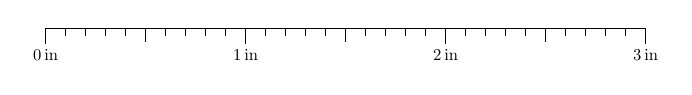
\begin{tikzpicture}
    \draw(0,0)--(3in,0); 
    \foreach \x in {0,1,2,3}{ 
        \draw (\x in,0) -- (\x in,-.2) node[below,scale=0.6]{\x\thinspace in}; 
    }  
    \foreach \x in {0.1,0.2,...,2.9}{       
        \draw (\x in,0) -- (\x in,-0.1); 
    }  
    \foreach \x in {0.5,1,...,2.5}{ 
        \draw (\x in,0) -- (\x in,-.17);  
    }
\end{tikzpicture}

 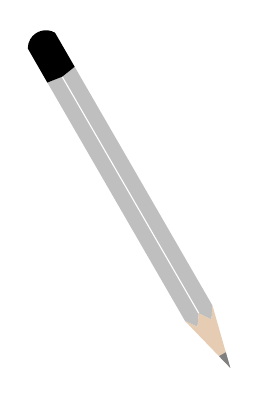
\begin{tikzpicture}[rotate=30]
            \fill[gray!50] (0,4) -- (0.4,4) -- (0.4,0) --(0.3,-0.15) -- (0.2,0) -- (0.1,-0.14) -- (0,0) -- cycle;
            \draw[color=white] (0.2,4) -- (0.2,0);
            \fill[black] (0,3.5) -- (0.2,3.47) -- (0.4,3.5) -- (0.4,4) arc(30:150:0.23cm);
            \fill[brown!40] (0,0) -- (0.2,-0.8)node[coordinate,pos=0.75](a){} -- (0.4,0)node[coordinate,pos=0.25](b){} -- (0.3,-0.15) -- (0.2,0) -- (0.1,-0.14) -- cycle;
            \fill[gray] (a) -- (0.2,-0.8) -- (b) -- cycle;
 \end{tikzpicture}
  
  \begin{tikzpicture}[rotate=-30,transform shape]
            \draw (-0.2,0) rectangle (15.5,1);
            %% lower divisions
            \foreach \x in {0,1,...,15}{
            \draw (\x,0) -- (\x,0.2)node[above,scale=0.4]{\x};
            }
            \foreach \x in {0.1,0.2,...,14.9}{
            \draw (\x,0) -- (\x,0.075);
            }
            \foreach \x in {0.5,1,...,14.5}{
            \draw (\x,0) -- (\x,0.15);
            }
            % Upper divisions
            \foreach \x in {0,1,...,6}{
            \draw (\x in,1) -- (\x in,0.8)node[below,scale=0.4]{\x};
            }
            \foreach \x in {0.1,0.2,...,5.9}{
            \draw (\x in,1) -- (\x in,0.925);
            }
            \foreach \x in {0.5,1,...,5.5}{
            \draw (\x in,1) -- (\x in,0.85);
            }
        \end{tikzpicture}
        
  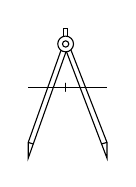
\begin{tikzpicture}[rotate=0,transform shape]
    %\draw[help lines] (0,0) grid (5,5);
       \draw (2.95,3.7) rectangle (3,3.95);
       \draw (2.92,3.68) -- (2.5,2.5) -- (2.5,2.3) -- (2.99,3.68);
       \draw (3.5,2.5) -- (3.43,2.48);
       \draw (3.04,3.68) -- (3.5,2.5) -- (3.5,2.3) -- (2.975,3.68);
       \draw (2.5,2.5) -- (2.56,2.48);
       \draw[fill=white] (2.975,3.75) circle (0.1cm);
       \draw (2.975,3.75) circle (0.04cm);
       \draw (2.5,3.2) -- (3.5,3.2);
       \draw[line width = 0.5pt,line cap=round] (2.975,3.15) -- (2.975,3.25);
\end{tikzpicture}       
\end{document}